\documentclass{article}


% if you need to pass options to natbib, use, e.g.:
%     \PassOptionsToPackage{numbers, compress}{natbib}
% before loading neurips_2023


% ready for submission
\usepackage[final, nonatbib]{neurips_2023}


% to compile a preprint version, e.g., for submission to arXiv, add add the
% [preprint] option:
%     \usepackage[preprint]{neurips_2023}


% to compile a camera-ready version, add the [final] option, e.g.:
%     \usepackage[final]{neurips_2023}


% to avoid loading the natbib package, add option nonatbib:
%    \usepackage[nonatbib]{neurips_2023}


\usepackage[utf8]{inputenc} % allow utf-8 input
\usepackage[T1]{fontenc}    % use 8-bit T1 fonts
\usepackage{hyperref}       % hyperlinks
\usepackage{url}            % simple URL typesetting
\usepackage{booktabs}       % professional-quality tables
\usepackage{amsfonts}       % blackboard math symbols
\usepackage{nicefrac}       % compact symbols for 1/2, etc.
\usepackage{microtype}      % microtypography
\usepackage{xcolor}         % colors

\usepackage[spanish, es-tabla]{babel}

\usepackage[pdftex]{graphicx}
\usepackage{subcaption}
\graphicspath{{./graphs/}}

%% biblatex
\usepackage[style = numeric, backend = biber, sorting = none, doi = false, isbn = false, url = true]{biblatex}
% \usepackage[defernumbers = true, style = numeric, backend = biber, sorting = none, doi = false, isbn = false, url = true]{biblatex}
% \usepackage[style = numeric, backend = biber, sorting = none]{biblatex}    % REFERENCIAS como section
\AtEveryBibitem{
    \clearfield{urlyear}
    \clearfield{urlmonth}
} % Do not show the "(visited on <date>)" on the references
\DefineBibliographyStrings{spanish}{}
\usepackage{csquotes}
\addbibresource{./dataminingCyT.bib}
\renewcommand*{\bibfont}{\fontsize{9}{12}\selectfont}



\title{Procesamiento de imágenes (pre TP1)}

\author{
  Víctor A.~Bettachini\\ %\thanks{Use footnote for providing further information about author (webpage, alternative address)---\emph{not} for acknowledging funding agencies.} \\
  Datamining en ciencia y tecnología 2023\\
  Especialización en Explotación de Datos y Descubrimiento del Conocimiento\\
  \texttt{bettachini@gmail.com}
}


\begin{document}


\maketitle


\begin{abstract}
Cuca.
\end{abstract}


% Enunciado
% Se sugiere realizar la entrega en formato latex, pero en este caso va a ser optativo (en el TP ya es obligatorio, sugerimos que lo usen de práctica). Pueden acceder a formatos de distintas conferencias a través de Overleaf, en particular les sugerimos el formato de NeurIPS que es una de las conferencias más importantes en IA.
% Se sugiere un máx de 4 carillas (mín 2), no se debe incluir código a menos que sea algo esencial que hayan desarrollado ustedes (es preferible en este caso incluir el pseudo-código). Aclaración: No vamos a corregir código en la entrega.
% El pre TP es individual.


\section{Introducción}
Cuca


\section{Materiales y métodos}

\paragraph{Datos}
210 imágenes de flores acompañados de un listado de las correspondientes especies dentro de una variedad de 10.
Las imágenes en formato png tienen una dimensión de 128 x 128 píxeles con tres canales de color.
El conjunto se descargó de una fuente pública \cite{belitskaya_flower_2020}.


\paragraph{Recurso informático} 
Un cuaderno (notebook) Jupyter provisto por los docentes en el sitio web denominado ``Campus'' \cite{kamienkowski_curso_2023} es la plantilla donde se escribió código en lenguaje Python.
Este explotó funciones de las bibliotecas OpenCV (\verb'cv2') y Clustimage para el trabajo con imágenes.
% Se modificó el sendero a los archivos para indicar un directorio en un sistema de archivos local de una computadora local para ejecutarle con mayor velocidad.


\section{Resultados}

\subsection{Preprocesamiento de los datos}
% Cada actividad realizada se describe bajo los titulos que figuran en el enunciado del trabajo práctico publicado en el

% Cargar el dataset y sus respectivas etiquetas. Es importante asegurarse que las imágenes sean comparables en color, valor, rango y tamaño.
\paragraph{Carga del conjunto de datos} 
La función \verb'cv2.imread' carga los canales es azúl, verde, rojo (BGR: blue, green, red).
Invertiendo la carga en un array (arreglo de la biblioteca numpy) se los ordena como RGB con la sentencia \verb'cv2.imread(path[0])[...,::-1]', en este caso para la primer imagen en el directorio al que apunta \verb'path'.
La \hyperref[fg:path0]{figura \ref*{fg:path0}} muestra en colores naturales la imagen generada a partir del array por la función \verb'imshow' de la biblioteca matplotlib.

% Explorar y graficar los subconjuntos de imágenes que representan flores de la misma especie



\subsection{Manipulación de datos}

% Cambiar la intensidad de una de las imágenes en escala de grises, transformarla en una imagen con mucho y otra con poco brillo.
\paragraph{Escala de grises}
Se utilizó la combinación lineal que preserva la luminancia perceptual de la codificación de color sRGB de la Commission Internationale de l'éclairage en 1931 según el consorcio W3 \cite{noauthor_standard_1996} $
Y_\mathrm{lineal} = 0.2126 R_\mathrm{lineal} + 0.7152 G_\mathrm{lineal} + 0.0722 B_\mathrm{lineal} .
$
La \hyperref[fg:imgGrau]{figura \ref*{fg:imgGrau}} muestra la luminancia obtenida en una escala lineal de grises.

Una alternativa a realizar esto manualmente es recurrir a la función \verb'cv2.cvtColor(img, cv2.COLOR_BGR2GRAY)'.
El producto es similar, como lo muestra el comparar histogamas de ambas alternativas (ver figura \hyperref[fg:grayHist]{figura \ref*{fg:grayHist}}).


\paragraph{Brillo}
Aplicar una función lineal 
$
Y_\mathrm{salida} = \alpha Y_\mathrm{entrada} + \beta ,
$
donde $\alpha$ la ganancia controla el contraste y $\beta$ el sesgo controla el brillo modifica el histograma de luminancia \cite{noauthor_opencv_nodate}.
Si \(beta \gg 0\) hace que \(Y_\mathrm{lineal final}> 255\) se les asigna este último valor.
Esto produce saturación (ver figura \hyperref[fg:saturada]{figura \ref*{fg:saturada}}).
Para evitar esto se utiliza una ley de potencias
\(
Y_\mathrm{salida} = 255 \left( \frac{Y_\mathrm{entrada}}{255} \right)^\gamma  
\)
conocida como corrección gamma por el exponente utilizado.
Un \(\gamma= .4\) redundó en la \hyperref[fg:imgGrau0p4exp]{figura \ref*{fg:imgGrau0p4exp}}, que muestra mayor brillo sin saturación (ver figura \hyperref[fg:grayHist]{figura \ref*{fg:brightHist}}).
Se reduce la luminancia con un \(\gamma >1\), como ejemplifica la \hyperref[fg:imgGrau3p5exp]{figura \ref*{fg:imgGrau3p5exp}} para \(\gamma = 3.5\).



% Convertir una de las imágenes a blanco y negro (binario). ¿Es la única manera? Si existen otras transformaciones mostrar más de una conversión.
\paragraph{Imágen binarizada}	
Se creó una matríz de ceros de la misma dimensión que la de luminancia.
A los píxeles con valores por sobre la mediana (\verb'statistics.median') se les asigno el valor unidad en la nueva matriz que se muestra en la \hyperref[fg:imgGrau0binarizada]{figura \ref*{fg:imgGrau0binarizada}}






% Recortar una parte significativa de la imagen, quedándose sólo con el círculo central de la misma.
\paragraph{Recorte circular}
Se generó un arreglo con tres matrices de ceros sobre las que se copiarian píxeles de la imagen original de cumplire una condición en función de un radio \(r\) del cuatro del número de columnas.
La condición define un círculo centrado con \((i- i_0)^2 + (j- j_0)^2 < r^2\) siendo \((i,j)\) e \((i_0, j_0)\) filas y columnas del arreglo y sus valores centrales respectivamente.
Aplicando la condición en los tres canales de color se obtuvo el viñetado con un círculo de diámetro mitad del ancho de la imágen que muestra la \hyperref[fg:circle]{figura \ref*{fg:circle}}. 


% Generar dos imágenes random: una imagen mezclando los pixels y otra mezclando partes de diferentes imágenes.

\paragraph{Aleatorizar imagen} Aleatorizar índices de píxeles a 
Copiar píxeles de la imagen original con \verb'imgAzar[i,j,c] = img[ indices[i*j][0], indices[i*j]' dentro de dos ciclos for anidados siendo \((i,j)\) los  de una lista aleatorizada produjo una imagen que visualmente muestra tener estructura (ver \hyperref[fg:alea1]{figura \ref*{fg:alea1}}.

La figura \hyperref[fg:alea2]{figura \ref*{fg:alea2}} muestra en este aspecto un mejor resultado.
Para lograrle se pasaron las valores para cada color en tres vectores y cuyos ordenemientos fueron simultáneamente cambiados al azar.
Luego se reconstruyeron las tres matrices en el orden original.

\begin{figure}
  \centering
	\begin{subfigure}[b]{0.24\textwidth}
		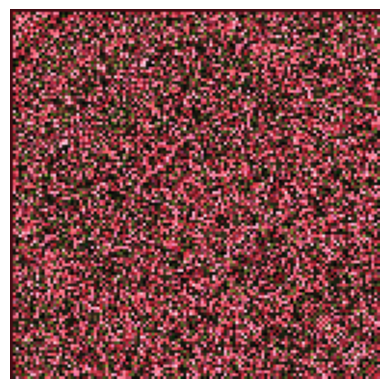
\includegraphics[width= \textwidth]{alea1}
		\caption{Reordenar índices}
		\label{fg:alea1}
	\end{subfigure}
	\begin{subfigure}[b]{0.24\textwidth}
		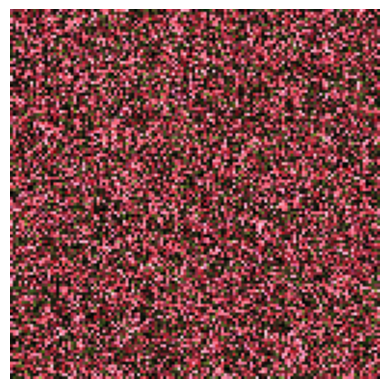
\includegraphics[width= \textwidth]{alea2}
		\caption{Mezclar píxeles}
		\label{fg:alea2}
	\end{subfigure}
	\caption{Procesamientos de la primer imagen en el conjunto de datos}
\end{figure}




% Aplicar dos tipos diferentes de filtros sobre una imagen, explique en qué casos conviene usar cada uno.

% Calcular imagen promedio global y el promedio entre las distintas especies. ¿Se pueden distinguir los promedios? ¿Cómo quedan los promedios si consideran las imágenes en blanco y negro?



\begin{figure}
  \centering
	\begin{subfigure}[b]{0.24\textwidth}
		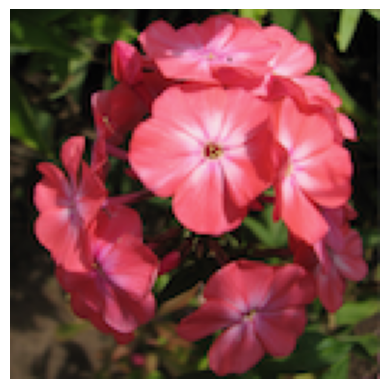
\includegraphics[width= \textwidth]{path0}
		\caption{Original}
		\label{fg:path0}
	\end{subfigure}
	\begin{subfigure}[b]{0.24\textwidth}
		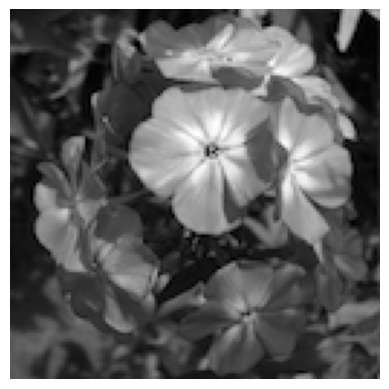
\includegraphics[width= \textwidth]{imgGrau}
		\caption{Solo luminancia}
		\label{fg:imgGrau}
	\end{subfigure}
	\begin{subfigure}[b]{0.24\textwidth}
		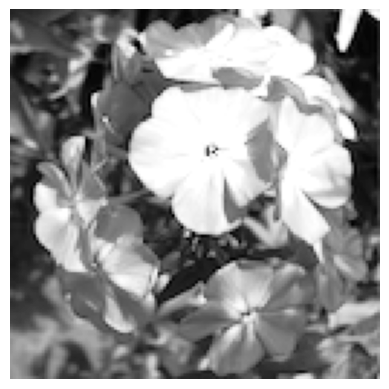
\includegraphics[width= \textwidth]{saturada}
		\caption{Saturada}
		\label{fg:saturada}
	\end{subfigure}
	\begin{subfigure}[b]{0.24\textwidth}
		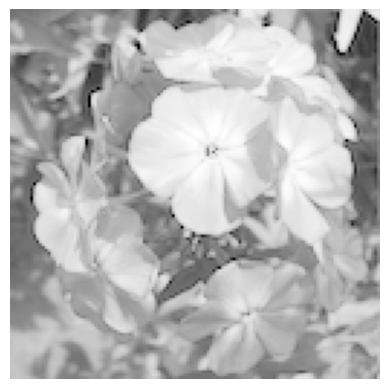
\includegraphics[width= \textwidth]{imgGrau0p4exp}
		\caption{Abrillantada}
		\label{fg:imgGrau0p4exp}
	\end{subfigure}
	\begin{subfigure}[b]{0.24\textwidth}
		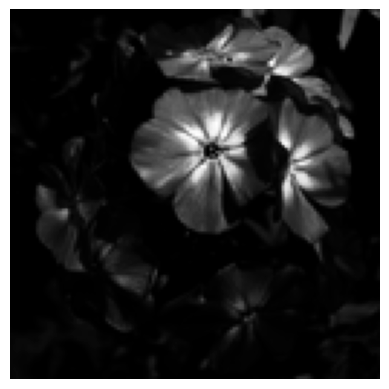
\includegraphics[width= \textwidth]{imgGrau3p5exp}
		\caption{Oscurecida}
		\label{fg:imgGrau3p5exp}
	\end{subfigure}
	\begin{subfigure}[b]{0.24\textwidth}
		
\includegraphics[width= \textwidth]{imgGrau0binarizada}
		\caption{Binarizada}
		\label{fg:imgGrau0binarizada}
	\end{subfigure}
	\begin{subfigure}[b]{0.24\textwidth}
		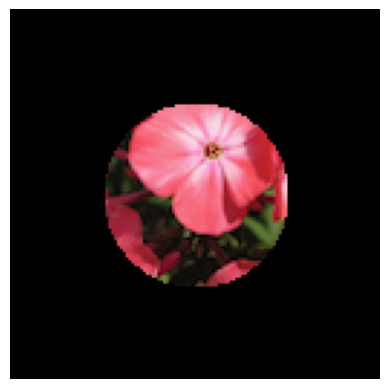
\includegraphics[width= \textwidth]{circle}
		\caption{Viñetado}
		\label{fg:circle}
	\end{subfigure}
	\caption{Procesamientos de la primer imagen en el conjunto de datos}
\end{figure}

\begin{figure}
  \centering
	\begin{subfigure}[b]{0.48\textwidth}
		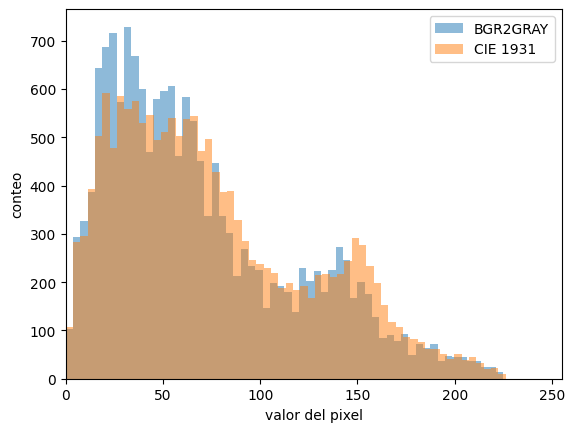
\includegraphics[width= \textwidth]{grayHist}
		\caption{Escala de grises.}
		\label{fg:grayHist}
	\end{subfigure}
	\begin{subfigure}[b]{0.48\textwidth}
		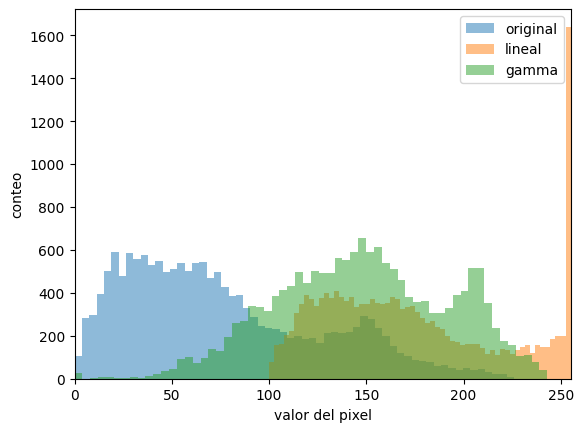
\includegraphics[width= \textwidth]{brightHist}
		\caption{Incremento brillo.}
		\label{fg:brightHist}
	\end{subfigure}
	\caption{Comparación de histogramas.}
\end{figure}



\subsection{Búsqueda de \emph{features}}

% Analizar las distribuciones de valores de pixels por cada especie. ¿Se puede distinguir una especie en algún rango de color?

% Realizar una inspección de las componentes principales del dataset y analizar si se pueden identificar las especies en esta representación.

\paragraph{Análisis de componentes principales}
Una centena de componentes principales por imagen se obtuvieron con el método \verb'exctract_feat' \cite{taskesen_pca_2020}.




\section{Discusión}

\begin{figure}
  \centering
  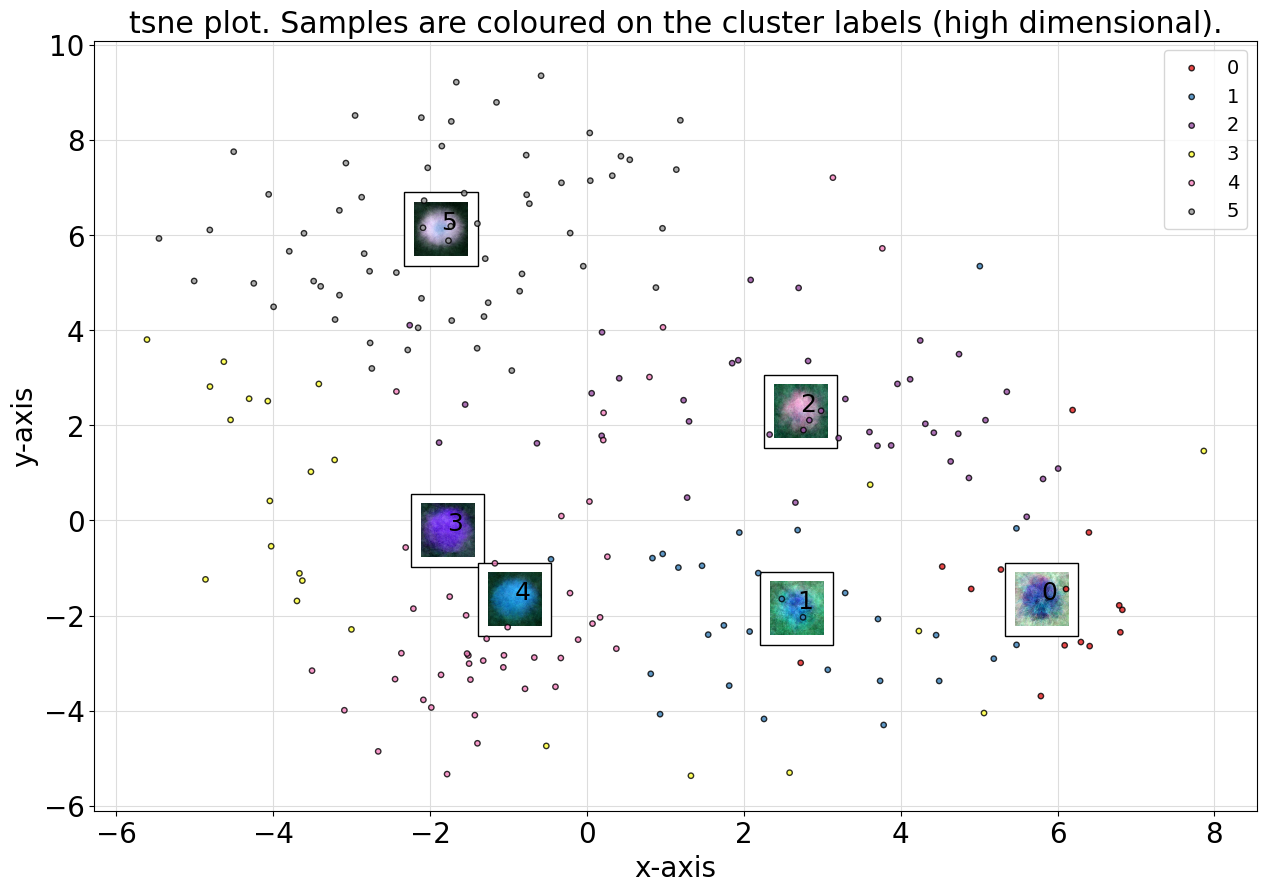
\includegraphics[width= 0.8\linewidth]{tsne}
  \caption{Ubicación de cada imágen en componentes principales(tsne plot)}
\end{figure}


\printbibliography[title= Referencias, heading=bibintoc]

\end{document}
